
Initial runs of the algorithm were performed on a two dimensional cellular culture. Its height was set to 0.768 mm while the width was fixed at 1.536 mm. The total number of supported and vascular cells were 4200 and 1800, respectively where vascular cells contributed to 30 per cent of total number of cells. A total of 384 circulatory cells simulating the external delivery and metabolic product extraction system is implemented as two identical columns on two sides of the cellular culture. The number of all mentioned cells were kept constant through the experiment. The simulations started with a random distribution of supported and vascular cells inside the culture. Sixteen simulated hours are allocated for network development, after which the network's quality is evaluated. If no path of vessels is found that connects the source to the sink, then the fitness score is set at zero. Otherwise, the fitness score of the network is estimated by measuring the metabolic productivity of the supported cells while simulating the operation of the vascular network for two simulated hours. This process is described in detail in Section~\ref{fitnessFunction}.


Figure~\ref{evolutions} shows the best case fitness of the networks produced during the running of the genetic algorithm. The algorithm starts with random values for the chosen parameter within the given ranges. As shown in the graph, the GA is unsuccessful in creating a productive cell culture for the first several evolutions. However, once it finds a parameter set leading to a functioning network, it continually improves the quality of solutions. After 1,000 iterations, the highest fitness level was 537.66 $\mu g$ of product production. The parameter values contributing to the best case are shown in Table~\ref{results}.

\begin{figure}[!t]
\centering
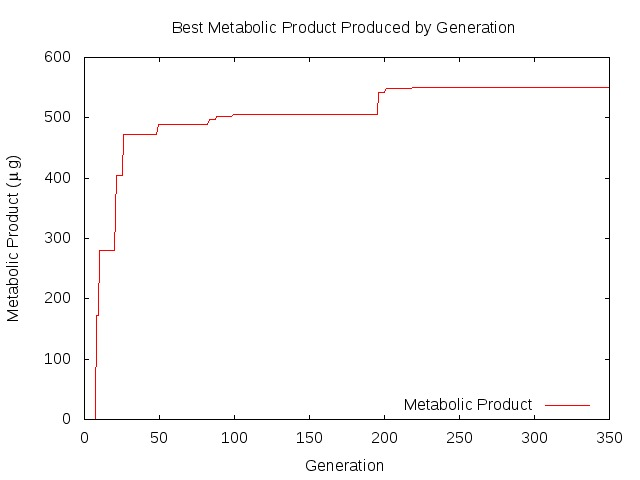
\includegraphics[width=3in]{./results/evolution products.jpg}

\caption{The metabolic production of the best-so-far individual identified as a function of generation. Only a single run is provided due to the four hours needed for each fitness evaluation.}
\label{evolutions}
\end{figure}



\begin{table}[ht]
\caption{The best parameter values found by the GA} % title of Table
\centering
\begin{footnotesize}
\begin{tabular}{l l l}
\hline

%\\ [1ex]      % [1ex] adds vertical space
$k$          & $6.78 \times 10^{-3}$                 & Monod-kinetic coefficient \\
$\mu_{short}$ & $5.12$                 & Secretion rate of $C_{short}$\\
$\mu_{long}$  & $6.10$                 & Secretion rate of $C_{long}$ \\
$\beta_{short} $    &  $67.3 \times 10^{-3}$         & Decay rate of $C_{short}$\\
$\beta_{long} $    &  $7.41 \times 10^{-6}$           & Decay rate of $C_{short}$\\
$\lambda_{short} $    &  $2.69$          & Chemoattractant response to $C_{short}$\\
$\lambda_{long} $    &  $1.99$           & Chemoattractant response to $C_{long}$\\
[1ex]      % [1ex] adds vertical space

\hline
\end{tabular}
\end{footnotesize}
\label{results}
\end{table}

\begin{figure*}[ht]
 \begin{center}
  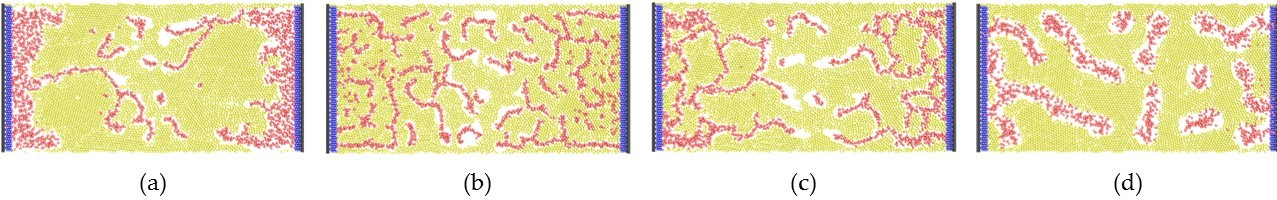
\includegraphics[width=\textwidth]{./results/bad factories.jpg}
 \end{center}
  \caption{Sample results of the GA during its evolution. These results show unsuccessful attempts of the GA at creating a consistent vascular network for the flow of nutrients and products}
\label{badFactories}
\end{figure*}

\begin{figure*}[ht]
 \begin{center}
  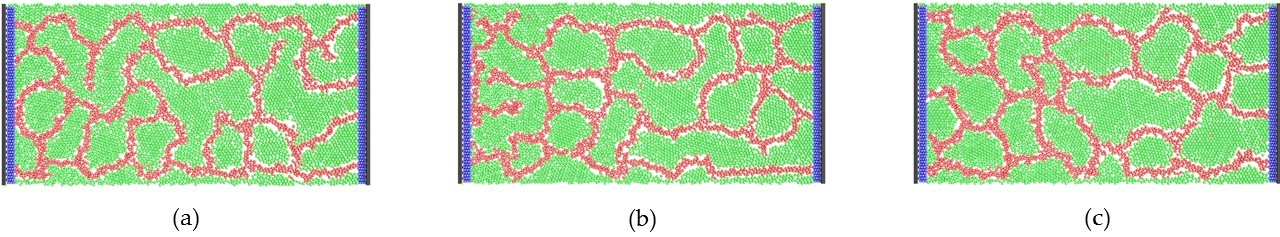
\includegraphics[width=\textwidth]{./results/good factories.jpg}
 \end{center}
  \caption{A sample of best solutions identified by the genetic algorithm during evolution. These results depict vascular networks that have successfully nourished the supported cells along with removing their products and waste}
\label{goodFactories}
\end{figure*}

Figure~\ref{badFactories} shows some sample cell cultures produced by the genetic algorithm during its evolution. As it is seen in the figure, some arrangements of the vascular cells do not form a network for the flow of material and thus no production is obtained in the system. Figure~\ref{badFactories}~(a) depicts a cell culture with most of the vascular cells accumulated beside the circulatory cells on the sides and occasional formations in the middle. This can be a result of high chemotactic response to $C_{long}$ and $\alpha$.

Figures~\ref{badFactories}~(b) and (d) both demonstrate scattered and disconnected lines of vascular cells floating among supported cells. Such arrangements result from a low amount of $C_{long}$ but a high amount of $\beta_{short}$. It should be mentioned that the cell culture in Figure~\ref{badFactories}~(d) has a higher $\beta_{short}$ than the one in ~\ref{badFactories}~(b) which accounts for the thicker lines of vascular cells. On the other hand, Figure~\ref{badFactories}~(c) shows another unsupported cell culture with several cycles of vascular cells but no path connecting the source to the sink. This result follows from low $\lambda_{short}$ and high $\lambda_{long}$ and $\mu_{long}$.

Figure~\ref{goodFactories} depicts cellular cultures found by the GA that have successfully formed networks of vascular cells and reached the highest amount of production. No patches of yellow non-producing cells are present in these cell cultures. As depicted, vascular cells have successfully formed a number of lacunae that feed all supported cells available in the culture and move waste and products away. More lacunae of vascular cells means availability of nutrients to more supported cells and therefore, higher production. Investigating the parameters leading to these solutions reveal an average amount of $\lambda_{short}$ and $\lambda_{long}$ and low amounts of $\mu_{short}$, $\mu_{long}$, $\beta_{short}$, $\beta_{long}$ and $k$. There are few unconnected branches stretching from a few points which given a larger time frame could lead to more lacunae and even a higher production. The exact amount of each parameter for cultures depicted in Figures~\ref{badFactories} is given in Table~\ref{figure-param-table}. For comparison purposes, the parameter values for Figure~\ref{goodFactories}(a) is also given in the same table.

\begin{table*}[t]
\renewcommand{\arraystretch}{1.3}
\caption{Parameter Table Corresponding to cellular cultures depicted in Figures~\ref{badFactories} and ~\ref{goodFactories}}
\label{figure-param-table}
\centering
\begin{tabular}{c||c||c||c||c||c||c||c}
\hline
\bfseries Culture  & \bfseries $\lambda_{short}$ & \bfseries $\lambda_{long}$ & \bfseries $\mu_{short}$ & \bfseries $\mu_{long}$ & \bfseries $\beta_{short} $ & \bfseries $\beta_{long}$ & \bfseries $k$ \\
\hline\hline
Figure~\ref{badFactories}-(a) & 1.28	& 4.09	& 5.90	& 6.58	& $6.79 \times 10^{-2}$ & $5.96 \times 10^{-4}$	& $2.64 \times 10^{-3}$\\
Figure~\ref{badFactories}-(b) & 1.28	& 5.92 &	5.90	& 5.21	& $6.79 \times 10^{-2}$ & $8.54 \times 10^{-4}$	& $8.96 \times 10^{-3}$\\
Figure~\ref{badFactories}-(c) & 1.11	& 1.22	& 6.69	& 4.50	& $9.90 \times 10^{-2}$	& $2.06 \times 10^{-4}$	& $1.49 \times 10^{-3}$\\
Figure~\ref{badFactories}-(d) & 5.73	& 1.22	& 6.69	& 4.50	& $8.14 \times 10^{-2}$	& $5.70 \times 10^{-4}$	& $2.17 \times 10^{-3}$\\
Figure~\ref{goodFactories}     & 2.69	& 1.34 & 	3.85  	& 6.10	&  	 	$3.23 \times 10^{-2}$ & $7.68 \times 10^{-5}$ &	$2.64 \times 10^{-4}$ \\
\hline
\end{tabular}
\end{table*}

